%%%%%%%%%%%%%%%%%%%%%%%%%%%%%%%%%%%%%%%%%
% Classicthesis-Styled CV
% LaTeX Template
% Version 1.0 (22/2/13)
%
% This template has been downloaded from:
% http://www.LaTeXTemplates.com
%
% Original author:
% Alessandro Plasmati
%
% License:
% CC BY-NC-SA 3.0 (http://creativecommons.org/licenses/by-nc-sa/3.0/)
%
%%%%%%%%%%%%%%%%%%%%%%%%%%%%%%%%%%%%%%%%%

%----------------------------------------------------------------------------------------
%	PACKAGES AND OTHER DOCUMENT CONFIGURATIONS
%----------------------------------------------------------------------------------------

\documentclass{scrartcl}

\reversemarginpar % Move the margin to the left of the page 

\newcommand{\MarginText}[1]{\marginpar{\raggedleft\itshape\small#1}} % New command defining the margin text style

\usepackage[utf8]{inputenc}
\usepackage[nochapters]{classicthesis} % Use the classicthesis style for the style of the document
\usepackage[LabelsAligned]{currvita} % Use the currvita style for the layout of the document
\usepackage{graphicx}

\renewcommand{\cvheadingfont}{\LARGE\color{Maroon}} % Font color of your name at the top

\usepackage{hyperref} % Required for adding links	and customizing them
\hypersetup{colorlinks, breaklinks, urlcolor=Maroon, linkcolor=Maroon} % Set link colors

\newlength{\datebox}\settowidth{\datebox}{Sep 2010-Aug 2011} % Set the width of the date box in each block

\newcommand{\NewEntry}[3]{\noindent\hangindent=2em\hangafter=0 \parbox{\datebox}{\small \textit{#1}}\hspace{1.5em} #2 #3 % Define a command for each new block - change spacing and font sizes here: #1 is the left margin, #2 is the italic date field and #3 is the position/employer/location field
\vspace{0.5em}} % Add some white space after each new entry

\newcommand{\Description}[1]{\hangindent=2em\hangafter=0\noindent\raggedright\footnotesize{#1}\par\normalsize\vspace{1em}} % Define a command for descriptions of each entry - change spacing and font sizes here

%----------------------------------------------------------------------------------------

\begin{document}

\thispagestyle{empty} % Stop the page count at the bottom of the first page

%----------------------------------------------------------------------------------------
%	NAME AND CONTACT INFORMATION SECTION
%----------------------------------------------------------------------------------------

\begin{cv}{\spacedallcaps{Matteo Facchini}}\vspace{1.5em} % Your name
	
\noindent\spacedlowsmallcaps{Personal Information}\vspace{0.5em} % Personal information heading

\MarginText{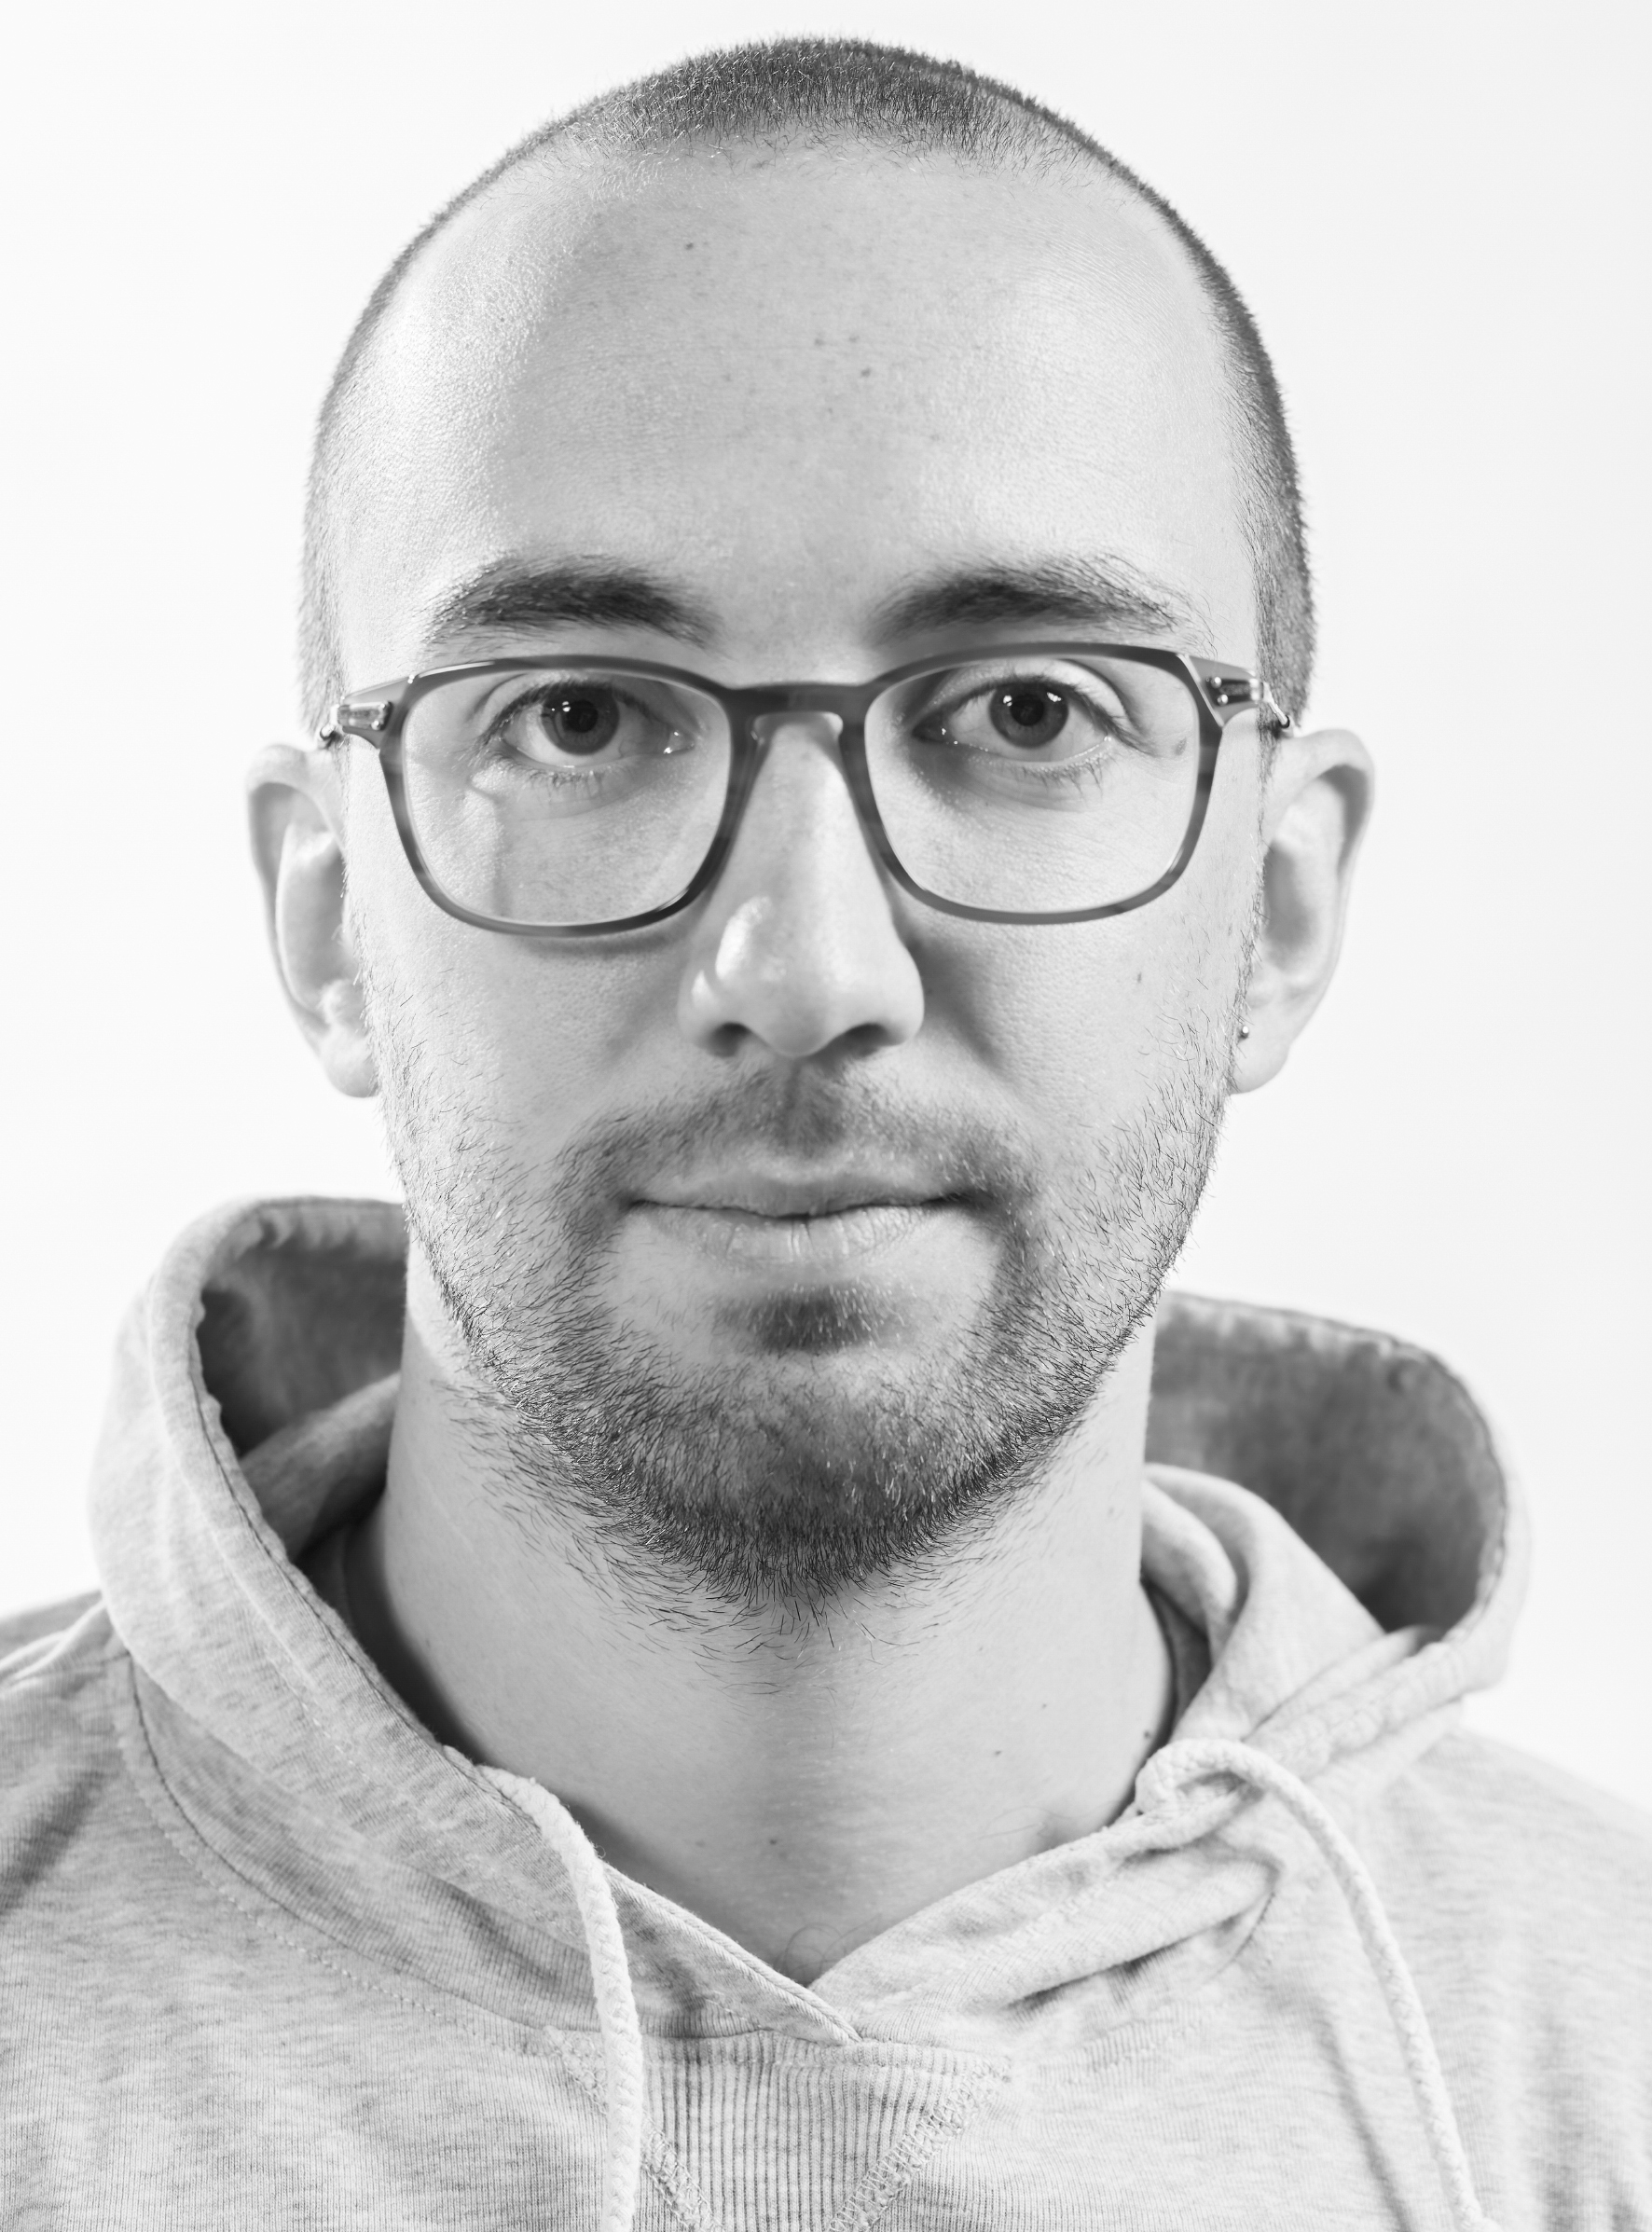
\includegraphics[width=3cm]{Facchini_Bild_2017_bw}}

\NewEntry{}{\textit{Born in Trento (Italy),}}{February 11, 1988} % Birthplace and date

\NewEntry{}{citizen of Italy} % citizenship

\NewEntry{address}{via vittime delle foibe, 40, I-38121, Trento} % Home address

\NewEntry{email}{\href{mailto:mat.facchini@gmail.com}{mat.facchini@gmail.com}} % Email address

\NewEntry{LinkedIn}{\href{https://www.linkedin.com/in/matteo-facchini-1098a393}{https://www.linkedin.com/in/matteo-facchini}}

\NewEntry{phone}{(U) +39 0461 282626 $\cdotp$\ \ (M) +39 340 230 4434} % Phone number(s)

\vspace{1em} % Extra white space between the personal information section and goal
%
%\noindent\spacedlowsmallcaps{Goal}\vspace{1em} % Goal heading, could be used for a quotation or short profile instead
%
%\Description{Gain fundamental experience in my area of interest and expertise.}\vspace{2em} % Goal text


%----------------------------------------------------------------------------------------
%	EDUCATION
%----------------------------------------------------------------------------------------

\spacedlowsmallcaps{Education}\vspace{1em}

\NewEntry{Nov 2013-Jan 2018}{ETH Zurich -- Zurich, Switzerland}

\Description{\MarginText{PhD}Laboratory of Hydraulics, Hydrology and Glaciology (VAW)\newline 
	Thesis: \textit{Downstream morphological effects of Sediment Bypass Tunnels}\newline 
	Description: monitoring and modeling the morphological effects of a sediment bypass tunnel (SBT) on the downstream river reach.\newline
	Advisors: Prof.~Robert M. \textsc{Boes} \& Dr.~Annunziato \textsc{Siviglia}}

%------------------------------------------------

\NewEntry{Oct 2010-Nov 2013}{Universit\`a degli Studi di Trento -- Trento, Italy}

\Description{\MarginText{Master Degree}Environmental and Land Engineering\newline 
Thesis: \textit{High order ADER-WENO finite volume schemes for Boussinesq-type equations}\newline
Advisor: Assoc. Prof.~Michael \textsc{Dumbser}}

%------------------------------------------------

\NewEntry{Sep 2011-Sep 2012}{Technische Univerität Dresden -- Dresden, Germany}

\Description{\MarginText{Erasmus Exchange}Civil and Environmental Engineering\newline}

%------------------------------------------------

\NewEntry{Sep 2007-Oct 2010}{Universit\`a degli Studi di Trento -- Trento, Italy}

\Description{\MarginText{Bachelor Degree}Environmental Engineering\newline
Thesis: \textit{Aspetti dei deflussi di pioggia: dilavamento di superfici stradali e rischi per i bacini limitrofi}\newline
Advisors: Assoc. Prof.~Sandra \textsc{Dirè} \& Assoc. Prof.~Maurizio \textsc{Righetti}}

%------------------------------------------------

\vspace{1em} % Extra space between major sections

%----------------------------------------------------------------------------------------
%	PRESENT APPOINTMENT
%----------------------------------------------------------------------------------------

%\noindent\spacedlowsmallcaps{Present appointment}\vspace{1em}
%
%\NewEntry{ - }{HM - Sustainable management of hydroelectric production, Hydropeaking Mitigation}
%
%\Description{\MarginText{HM}Free University of Bozen\newline 
%	Description: morphological mitigation measures assessment through development of a 3D fluid dynamic model coupled with physical habitat suitability model..\newline
%	Advisor: Prof.~Maurizio \textsc{Righetti}}
%
%\vspace{1em} % Extra space between major sections

%----------------------------------------------------------------------------------------
%	WORK EXPERIENCE
%----------------------------------------------------------------------------------------

\noindent\spacedlowsmallcaps{Work Experience}\vspace{1em}

\NewEntry{May 2018-May 2019}{Research Fellow, \textsc{University of Trento} -- Trento, Italy}

\Description{\MarginText{UniTN}Modeling of the effects of repeated sediment releases to glacier-fed gravel bed rivers.}

%------------------------------------------------

\NewEntry{Nov 2013-Jan 2018}{PhD Candidate, \textsc{ETH Zurich} -- Zurich, Switzerland}

\Description{\MarginText{ETH Zurich}Monitoring and modeling of downstream effects of Sediment Bypass Tunnel (SBT) releases at an alpine stream.}

%------------------------------------------------

\NewEntry{Nov 2013-Oct 2017}{Software Developer, \textsc{ETH Zurich} -- Zurich, Switzerland}

\Description{\MarginText{ETH Zurich}Software development of BASEMENT (Basic Simulation Environment for Computation of Environmental Flow and Natural Hazard Simulation), a software used in river engineering and morphodynamics modeling.}

%------------------------------------------------
%\pagebreak
\NewEntry{Jan-Mar 2013}{Faculty Advisor, \textsc{LEONARDO Formazione e Sviluppo} -- Catania, Italy}

\Description{\MarginText{LEONARDO}Tutoring students going to simulate a session of the United Nations (National Model United Nations, NMUN) in New York.}

%------------------------------------------------
%
%\NewEntry{Sep 2010-Aug 2011}{Sound and Lights Technician, \textsc{Opera Universitaria} --- Trento, Italy}
%
%\Description{\MarginText{Op. Univ. TN}Sound and light technician at Opera Universitaria cultural events, such as theater, concerts and movies.}

%%%------------------------------------------------
%
%\NewEntry{2005--2007}{Employee, \textsc{Istituto Comprensivo Trento 3} --- Trento (Italy)}
%
%\Description{\MarginText{Ist. Comp. TN3}Data implementation: results of assessment questionnaires concerning teaching quality at the institute.}

%------------------------------------------------

%\vspace{1em} % Extra space between major sections
\pagebreak
%----------------------------------------------------------------------------------------
%	PUBLICATIONS
%----------------------------------------------------------------------------------------

\spacedlowsmallcaps{Publications}\vspace{1em}

\Description{\MarginText{2019}
	M. \textsc{Facchini}, ~R.M. \textsc{Boes}, ~D.F. \textsc{Vetsch}, ~A.\textsc{Siviglia} (2018), Riverbed and surface composition adjustments in a gravel-bed river subject to repeated Sediment Bypass Tunnel operations, under review}

%------------------------------------------------

\Description{\MarginText{2018}
	M. \textsc{Facchini}, (2018), Downstream morphological effects of Sediment Bypass Tunnels, VAW Mitteilungen 243 (R.M. Boes ed.), ETH Zurich, Switzerland.}

%------------------------------------------------

\Description{\MarginText{2017}
	M. \textsc{Facchini}, ~A. \textsc{Siviglia}, ~R. M. \textsc{Boes}, (2017), Downstream morphological effects of SBT releases: 1D numerical study and preliminary LiDAR data analysis, In Proceedings of the 2$^{nd}$ International Workshop on Sediment Bypass Tunnels (T. Sumi ed.), Kyoto University, Kyoto, Japan.}

%------------------------------------------------

\Description{\MarginText{2016}
	M. \textsc{Dumbser}, ~M. \textsc{Facchini}, (2016), A space-time discontinuous Galerkin method for Boussinesq- type equations, Applied Mathematics and Computation, 272(2): 336-346.}

%------------------------------------------------

\Description{\MarginText{2015}
	M. \textsc{Facchini}, ~A. \textsc{Siviglia}, ~R.M. \textsc{Boes}, (2015), Downstream morphological impact of a sediment bypass tunnel – preliminary results and forthcoming actions, Proc. First International Workshop on Sediment Bypass Tunnels, VAW Mitteilungen 232, ETH Z\"urich, Schweiz, 137-146.}

%------------------------------------------------

\vspace{1em} % Extra space between major sections

%----------------------------------------------------------------------------------------
%	CONFERENCES AND COURSES
%----------------------------------------------------------------------------------------

\spacedlowsmallcaps{Conferences, Courses and Seminars:}\vspace{1em}

\Description{\MarginText{2018}American Geophysical Union (AGU) Fall Meeting -- Washington DC, USA -- December 11 - December 15 2018.}

\Description{\MarginText{}Seminar at St. Anthony Falls Laboratory -- Minneapolis, USA -- December 4 2018.}

\Description{\MarginText{2017}Second International Workshop on Sediment Bypass Tunnels -- Kyoto, Japan -- May 9 - May 12, 2017.}

\Description{\MarginText{2016}Summer School on Fluvial Geomorphology -- Losone, Switzerland -- June 27 - July 1, 2016.}

\Description{\MarginText{2015}Introduction to Writing at Doctoral Level, Natural Science \& Engineering, C1 level -- Zurich, Switzerland -- Fall Semester 2015.}

\Description{\MarginText{}International Workshop on Sediment Bypass Tunnels -- Zurich, Switzerland -- April 27 - April 29, 2015.}

\Description{\MarginText{2014}European Geoscience Conference General Assembly -- Vienna, Austria-- April 27- May 2, 2014.}

\Description{\MarginText{}Post-graduate Course on Advanced Numerical Methods for Hyperbolic Equations and Applications -- Trento, Italy -- February 3 - February 14, 2014.}

\Description{\MarginText{}Post-graduate Course on Basic Interdisciplinary River Morphodynamics: First Edition, River Bars -- Trento, Italy -- October 27 - October 31, 2014.}

%------------------------------------------------

\vspace{1em} % Extra space between major sections

%----------------------------------------------------------------------------------------
%	PERSONAL SKILLS
%----------------------------------------------------------------------------------------

\spacedlowsmallcaps{Language Skills}\vspace{1em}

\vspace{1em}

\newlength{\langbox} % Create a new length for the length of languages to keep them equally spaced
\settowidth{\langbox}{English} % Length equals the length of "English" - if you have a longer language in your list put it here

\Description{\MarginText{Mother tongue}\parbox{\langbox}{\textsc{Italian}}}

\vspace{-0.5em} % Negative vertical space to counteract the vertical space between every \Description command

\Description{\MarginText{Other languages}\parbox{\langbox}{\textsc{English}}\vspace{0.2em}
\begin{tabular}{ c c c c c }
	\multicolumn{2}{c}{UNDERSTANDING} & \multicolumn{2}{c}{SPEAKING} & WRITING \\
	Listening & Reading & Spoken interaction & Spoken production &  \\
	C1 & C1 & C1 & C1 & C1 \\
\end{tabular}
}
\Description{\parbox{\langbox}{\textsc{German}}\vspace{0.2em}	
	\begin{tabular}{ c c c c c }
		\multicolumn{2}{c}{UNDERSTANDING} & \multicolumn{2}{c}{SPEAKING} & WRITING \\
		Listening & Reading & Spoken interaction & Spoken production &  \\
		C1 & C1 & C1 & C1 & C1 \\
	\end{tabular}
}
\pagebreak
\Description{\MarginText{Communication and social skills}public speaking skills.
\vspace{0.5em}
\newline
didactic skills.
\vspace{0.5em}
\newline
team work orientation.
\vspace{0.5em}
\newline
taking on responsibilities.}

\Description{\MarginText{Organizational skills}ability of dealing with  conflicting priorities and multiple tasks.
\vspace{0.5em}
\newline
working experience in events organization and planning, for medium events (concerts and the Trento Masquerade Ball 2013).}

\Description{\MarginText{Job-related skills}good experience in the field of river monitoring by means of direct field measurements (GIS data sampling with mobile mapping, grain size distributions, flow speed measurements, topography, etc.) and remote measurements (airborne photogrammetry, 3D laser scanning by means of Laser Imaging Detection and Ranging (LiDAR)).
\vspace{0.5em}
\newline
good knowledge in the field of habitat evaluation and modeling of fluvial systems (MesoHABSIM methodology for morphological units classification).
\vspace{0.5em}
\newline
very good knowledge of Geographic Information Systems (GIS) applied to the evaluation of river topographic changes, i.e. of digital elevation models (DEM) evolution.
\vspace{0.5em}
\newline
very good knowledge of HydroVISH, a software developed by the company AHM (Innsbruck) used to classify clouds of points measured during LiDAR surveys.
\vspace{0.5em}
\newline
perfect knowledge of BASEMENT, a software developed at VAW (ETH Zurich), used for river engineering and morphodynamic modeling.}

\Description{\MarginText{Technology-related skills}very good knowledge of different operative systems (Macintosh, Windows and Ubuntu) and of their basic applications (e.g. iWork, Microsoft Office and LibreOffice).
\vspace{0.5em}
\newline
excellent knowledge of programming and scripting languages such as Python and Matlab; regular use on a daily basis of GitHub.
\vspace{0.5em}
\newline
good knowledge of programming and scripting languages such as C++, Fortran and R.
\vspace{0.5em}
\newline
basic knowledge of Docker and other softwares used in the engineering and mathematical fields such as Maple, HecRas, Ansys CFX e Comsol Multiphysics.}

\Description{\MarginText{Artistic skills}\parbox{\langbox}{\textsc{Music}}\ \ $\cdotp$\ \ \ percussions degree at the music school "I Minipolifonici" di Trento; several years of concert activity with the orchestra "I Filarmonici" di Trento (classical music), with the orchestras TU-Sinfonieorchester e TU-Kammerphilharmonie of the TU Dresden (classical music), with the marching band Corpo Musicale Citt\`a di Trento (classical and folk music) and in local bands (rock, blues, and funky music).}

\Description{\MarginText{Other skills}board member at the orchestra "I Filarmonici" di Trento until 2013.
\vspace{0.5em}
\newline
board member at the Corpo Musicale Citt\`a di Trento until 2013.
\vspace{0.5em}
\newline
member of the artistic board at the Corpo Musicale Citt\`a di Trento until 2013.
\vspace{0.5em}
\newline
students delegate at the high school Liceo Scientifico Statale "G. Galilei" di Trento during school years 2005-2006 e 2006-2007.
\vspace{0.5em}
\newline
students delegate in the Department Council at the Department of Civil, Environmental and Mechanical Engineering of the Università degli Studi di Trento during the academic year 2010-2011.}
%%------------------------------------------------
%
%\Description{\MarginText{Interests}Percussions\ \ $\cdotp$\ \ Music\ \ $\cdotp$\ \ Sports\ \ $\cdotp$\ \ Reading\ \ $\cdotp$\ \ Movies}

%----------------------------------------------------------------------------------------

\end{cv}

\end{document}